\documentclass[12pt]{article}

\usepackage[utf8]{inputenc}
\usepackage{amsmath,amssymb,hyperref,array,xcolor,multicol,verbatim,mathpazo}
\usepackage[normalem]{ulem}
\usepackage[pdftex]{graphicx}
\usepackage{fullpage}

\usepackage{threeparttable}
\usepackage{geometry}
\usepackage[format=hang,font=normalsize,labelfont=bf]{caption}
\usepackage{lscape}
\usepackage{natbib}
\usepackage{setspace}
\usepackage{float,color}
\usepackage[pdftex]{graphicx}
\usepackage{pdfsync}
\usepackage{placeins}
\usepackage{geometry}
\usepackage{pdflscape}
\usepackage[normalem]{ulem}
\usepackage{threeparttable, multirow}
\useunder{\uline}{\ul}{}
\synctex=1
\usepackage{hyperref}
\hypersetup{colorlinks,linkcolor=red,urlcolor=blue,citecolor=blue}
\usepackage{bm}


\newcommand{\E}{\mathbb{E}}

% Identifying information
\title{
Homework 4 Answers
} 
\author{Linghui Wu
\thanks{Solutions were discussed with Jiahui Shui.}
}
\date{\today}

\begin{document}

\maketitle

\section{Productivity Shocks in the Three Equation Model}

\subsection*{(a)}

Firstly, from 
\begin{align*}
\hat{a}_{t} &= \rho_{a} \hat{a}_{t-1} + \varepsilon_{t},
\end{align*}
we have 
\begin{align*}
\E_{t}\left[\hat{a}_{t+1}\right] &= \rho_{a}\hat{a}_{t}.
\end{align*}
The system of equations that characterizes the log-linearized NK model is
\begin{equation}
\label{eq:y_t}
\hat{y}_{t} = -\sigma\left(\hat{i}_{t}-\E_{t}\left[\hat{\pi}_{t}\right]\right) + \E_{t}\left[\hat{y}_{t+1}\right]
\end{equation}
\begin{equation}
\label{eq:pi_t}
\hat{\pi}_{t} = \kappa \left(\hat{y}_{t}-\frac{1+\phi}{\gamma+\phi}\hat{a}_{t}\right) + \beta\E_{t}\left[\hat{\pi}_{t+1}\right]
\end{equation}
\begin{equation}
\label{eq:i_t}
\hat{i}_{t} = \phi_{\pi}\hat{\pi}_{t}
\end{equation}
Using the method of undetermined coefficients, we assume that 
\begin{align*}
\hat{y}_{t} &= \eta_{ya}\hat{a}_{t} \\
\hat{\pi}_{t} &= \eta_{\pi a}\hat{a}_{t} \\
\hat{i}_{t} &= \eta_{ia}\hat{a}_{t}
\end{align*}
By simple algebra, equations (\ref{eq:y_t}), (\ref{eq:pi_t}) and (\ref{eq:i_t}) can be re-arranged as 
\begin{equation}
\label{eq:eta_ya}
\eta_{ya} = \frac{\sigma \left(\eta_{\pi a}\rho_{a}-\eta_{ia}\right)}{1-\rho_{a}}
\end{equation}
\begin{equation}
\label{eq:eta_pia}
\eta_{\pi a} = \frac{\kappa\left(\eta_{ya} - \frac{1+\varphi}{\gamma+\varphi}\right)}{1-\beta\rho_{a}}
\end{equation}
\begin{equation}
\label{eq:eta_ia}
\eta_{ia} = \phi_{\pi}\eta_{\pi a}
\end{equation}
Combining equations (\ref{eq:eta_ya}), (\ref{eq:eta_pia}) and (\ref{eq:eta_ia}),
we can pin down the three unknown coefficients
\newcommand{\etapia}{\frac{\kappa\left(1-\rho_{a}\right)\left(1+\varphi\right)}{\left(\gamma+\varphi\right)\left[\kappa\sigma\left(\rho_{a}-\phi_{\pi}\right)-\left(1-\rho_{a}\right)\left(1-\beta\rho_{a}\right)\right]}}
\begin{align*}
\eta_{ya} &= \frac{\sigma\left(\rho_{a}-\phi_{\pi}\right)}{1-\rho_{a}} \etapia \\
\eta_{\pi a} &= \etapia \\
\eta_{ia} &= \phi_{\pi}\etapia 
\end{align*}
Therefore, 
\begin{align*}
\hat{y}_{t} &= \frac{\sigma\left(\rho_{a}-\phi_{\pi}\right)}{1-\rho_{a}} \etapia \hat{a}_{t} \\
\hat{\pi}_{t} &= \etapia \hat{a}_{t} \\
\hat{i}_{t} &= \phi_{\pi}\etapia \hat{a}_{t}
\end{align*}

\subsection*{(b)}

By Fisher equation that $\E_{t}\left[R_{t+1}\right]=\E_{t}\left[Q_{t}\frac{P_{t}}{P_{t+1}}\right]$, we can derive
\begin{align*}
\hat{r}_{t} &= \hat{i}_{t} - E_{t}\left[\hat{\pi}_{t+1}\right] = \hat{i}_{t} - \eta_{\pi a}\rho_{a}\hat{a}_{t},
\end{align*}
and
\begin{align*}
\E_{t}\left[\hat{r}_{t+1}\right] &= \rho_{a}\left(\eta_{ia} - \eta_{\pi a}\rho_{a}\right) \hat{a}_{t}.
\end{align*}

\subsection*{(c)}

Figure \ref{fig:q1_irf} plots the impulse response functions.

Intuitively, a positive TFP shock decreases the marginal costs of the firm in the economy and increases the ``natural'' level of production in the frictionless economy. 
\begin{itemize}
    \item $\hat{a}_{t}$: It reflects the specified $AR(1)$ process.
    \item $\hat{y}^{flex}_{t}$: An increase in TFP raises the ``natural'' level of production in the unconstrained economy by making firms more productive.
    \item $\hat{y}_{t}$: Since some firms in the actual economy are constrained due to nominal rigidities, the rise in output in the actual economy is less than that in an unconstrained economy.
    \item $\hat{y}_{t}-\hat{y}^{flex}_{t}$: Putting the two points above yields a negative output gap, because the frictionless economy experiences a larger positive deviation from the steady state than the actual economy. 
    Mathematically, we have
    \begin{align*}
    \hat{mc}_{t} &= \left(\varphi+\gamma\right)\left(\hat{y}_{t}-\hat{y}^{flex}_{t}\right)
    \end{align*}
    \item $\hat{n}_{t}$: Employment decreases because firms do not need as much labor to produce their output. Mathematically, we have
    \begin{align*}
    \hat{y}_{t} &= \hat{a}_{t} + \hat{n}_{t}.
    \end{align*}
    \item $\hat{\pi}_{t}$: As the marginal costs decrease, firm can set lower prices to make the same level of profits, so the optimal reset price becomes smaller. This results in lower prices in the economy and thus inflation goes down.
    \item $\hat{i}_{t}$: Central Bank reacts to the decreasing inflation rate by reducing the nominal interest rate.
    \item $\E_{t}\left[\hat{r}_{t+1}\right]$: The real interest rate change is a devation from the nominal interest rate change by expected change in inflation, $\hat{r}_{t} = \hat{i}_{t} - E_{t}\left[\hat{\pi}_{t+1}\right]$. Since $\phi_{\pi}=1.5$, the real interest rate decreases.
\end{itemize}

\begin{figure}[ht]
\centering
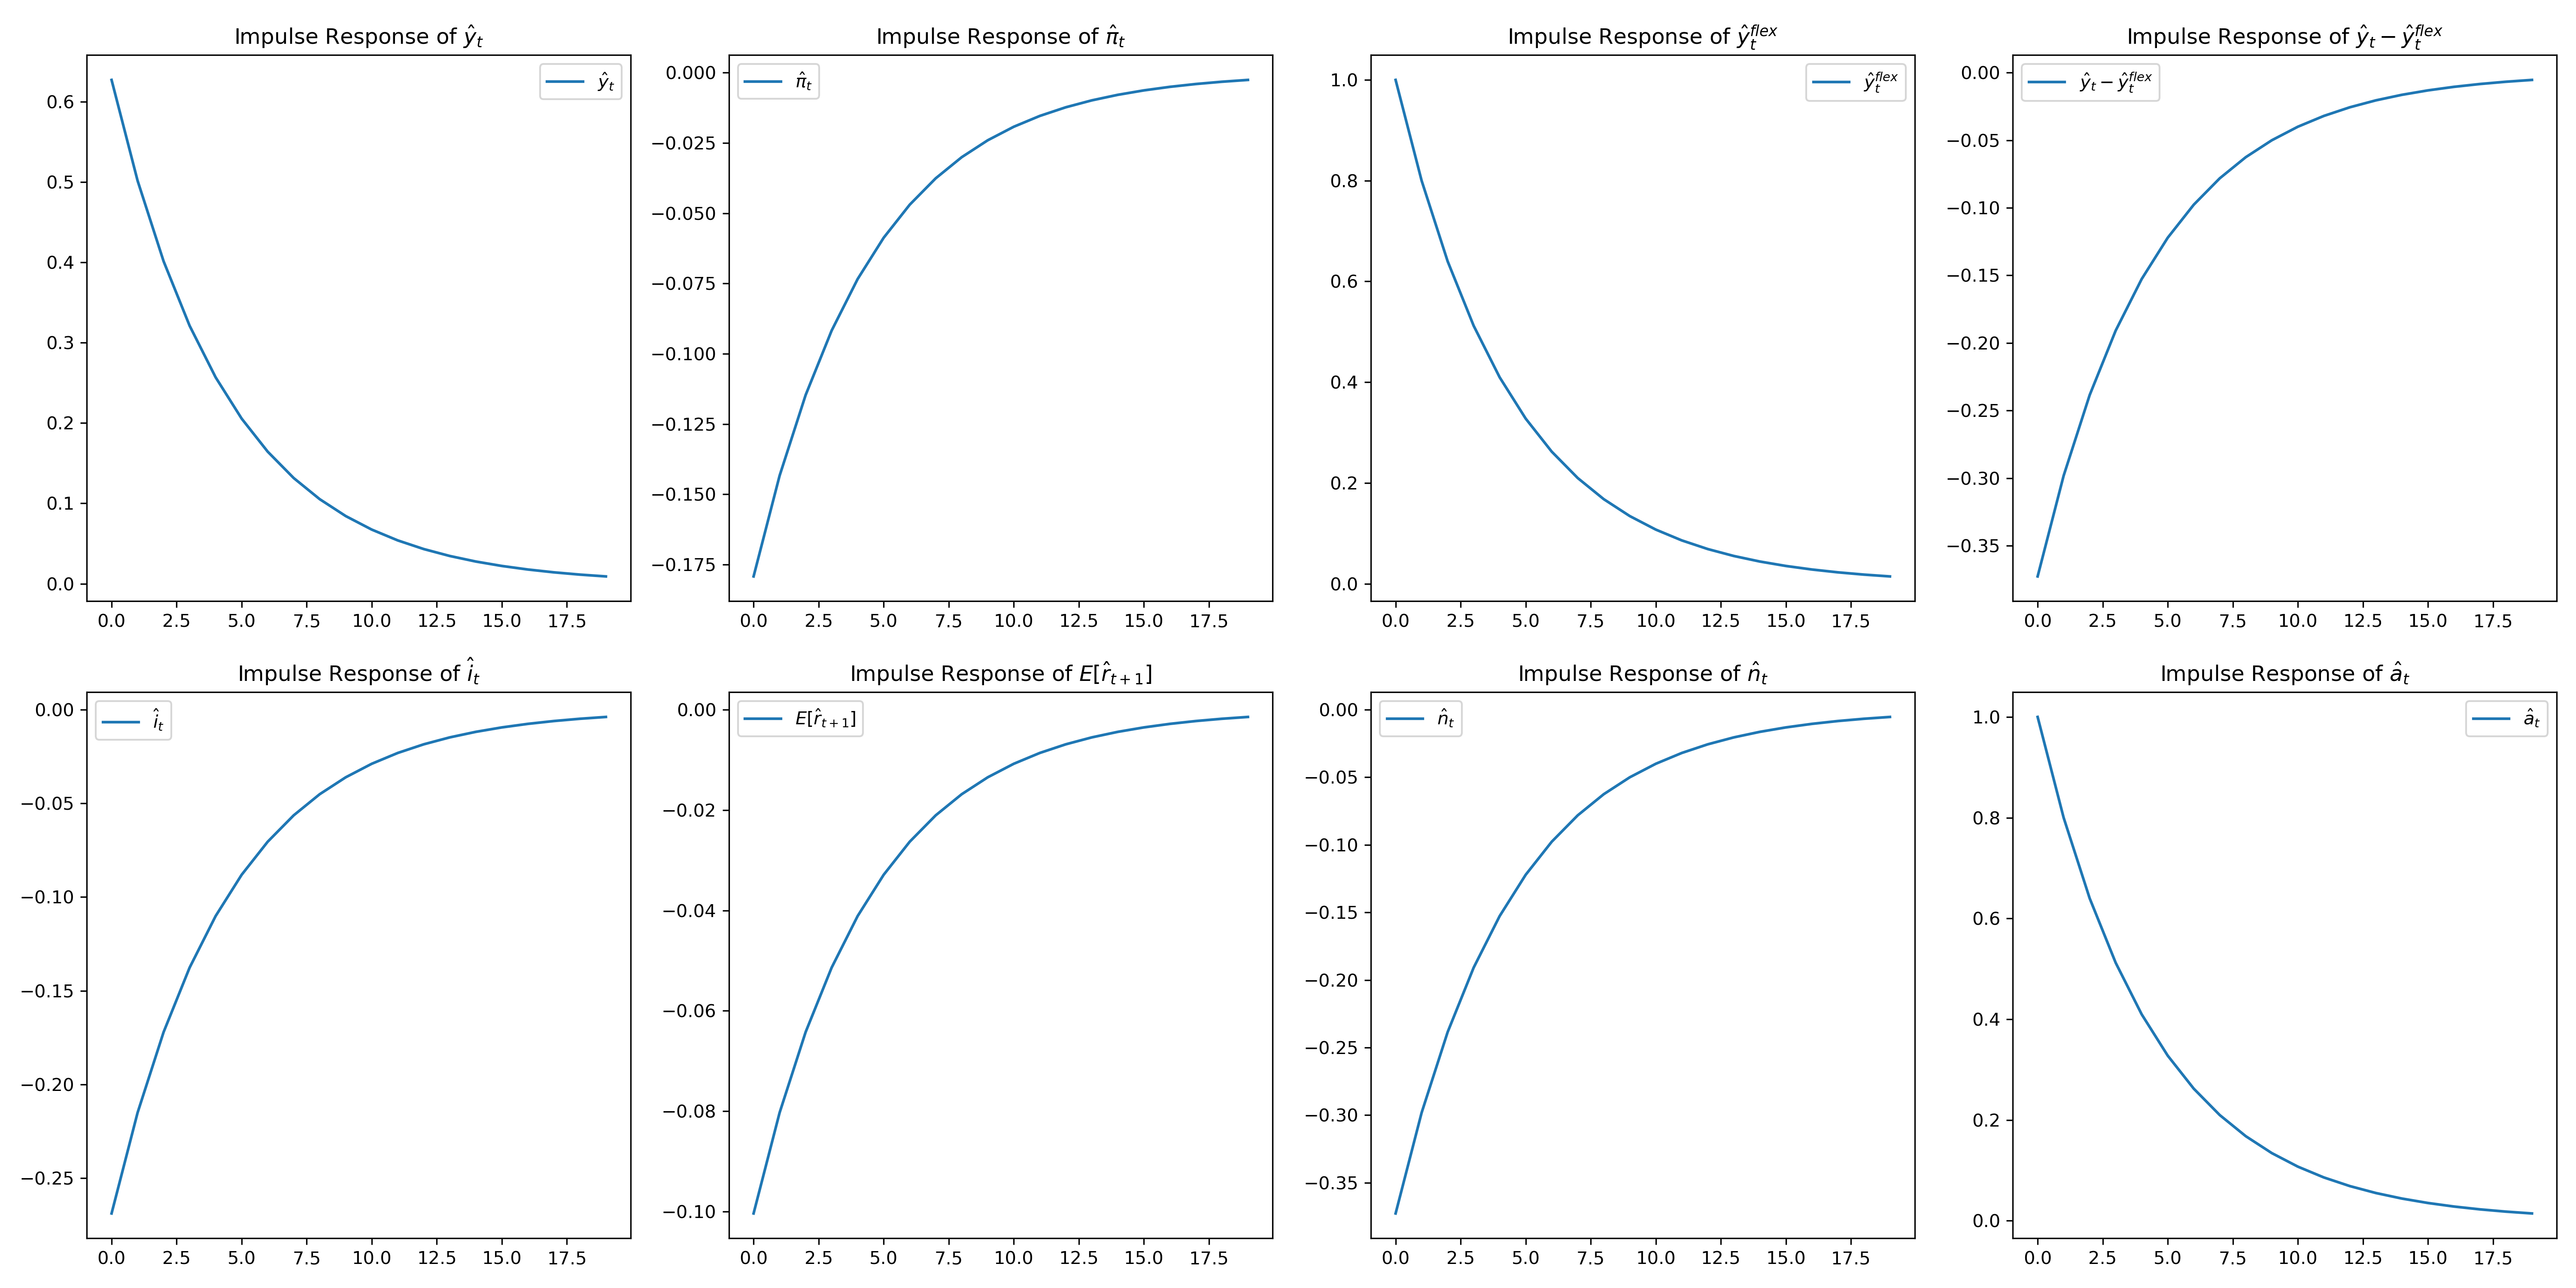
\includegraphics[width=0.8\textwidth]{figs/q1_IRFs.png}
\caption{Impulse Response Functions}
\label{fig:q1_irf}
\end{figure}

\subsection*{(d)}

The impulse responses in figure \ref{fig:q1_irf} are comparable to those in \texttt{newkeysianlinear.ipynb}.

\section{Non-linear NK Model in Jupyter}

\subsection*{(a)}

Mathematically, this expression is not recursive because it does not contain $P^{\ast}_{t+s} \forall s \in \mathbb{N}$. 
This is because the objective function for the intermediate producer's optimal reset pricing 
only puts weight on states of the world in which the price they set remains $P^{\ast}_{t}$ forever. 

Intuitively, when a firm gets to reset its price, its history does not matter,
which indicates that previous price-setting decisions do not affect future reset prices. 

\subsection*{(b)}

We are given 
\begin{equation}
\label{eq:lambda}
\Lambda_{t,t+k} = \Lambda_{t,t+1}\Lambda_{t+1,t+k} \forall
\end{equation}
\begin{equation}
\label{eq:F2}
F_{2,t} = \Sigma^{\infty}_{k=0}\theta^{k}\Lambda_{t,t+k}Y_{t+k}\left(\frac{P_{t+k}}{P_{t}}\right)^{\epsilon-1}.
\end{equation}
Iterating forward equation (\ref{eq:F2}) by one period, we have
\begin{equation}
\label{eq:F2prime}
F_{2,t+1} = \Sigma^{\infty}_{k=0}\theta^{k}\Lambda_{t+1,t+k+1}Y_{t+k+1}\left(\frac{P_{t+k+1}}{P_{t+1}}\right)^{\epsilon-1}.
\end{equation}
So,
\begin{align*}
F_{2,t} &= \theta^{0}\Lambda_{t,t}Y_{t} + \Sigma^{\infty}_{k=1} \theta^{k}\Lambda_{t,t+k}Y_{t+k}\left(\frac{P_{t+k}}{P_{t}}\right)^{\epsilon-1} \\
&= Y_{t} + \Sigma^{\infty}_{k=0} \theta^{k+1}\Lambda_{t,t+k+1}Y_{t+k+1}\left(\frac{P_{t+k+1}}{P_{t}}\right)^{\epsilon-1} \\
&= Y_{t} + \theta \Sigma^{\infty}_{k=0} \theta^{k}\Lambda_{t,t+1}\Lambda_{t+1,t+k}Y_{t+k+1}\left(\frac{P_{t+k+1}}{P_{t+1}}\frac{P_{t+1}}{P_{t}}\right)^{\epsilon-1} \\
&= Y_{t} + \theta\left(\Pi_{t+1}\right)^{\epsilon-1}\Lambda_{t,t+1}F_{2,t+1}.
\end{align*}

\subsection*{(c)}

By a similar argument as in part (b), we have
\begin{align*}
\label{eq:F1}
F_{1,t} &=\left(1+\mu\right)\Sigma^{\infty}_{s=0}\theta^{s}\Lambda_{t,t+s}Y_{t+s}\left(\frac{P_{t+s}}{P_{t}}\right)^{\epsilon-1}\frac{W_{t+s}}{P_{t}A_{t+s}} \\
&= \left(1+\mu\right)Y_{t}\frac{W_{t}}{P_{t}A_{t}} + \left(1+\mu\right)\Sigma^{\infty}_{s=1}\theta^{s}\Lambda_{t,t+s}Y_{t+s}\left(\frac{P_{t+s}}{P_{t}}\right)^{\epsilon-1}\frac{W_{t+s}}{P_{t}A_{t+s}} \\
&= \left(1+\mu\right)Y_{t}\frac{W_{t}}{P_{t}A_{t}} + \left(1+\mu\right)\Sigma^{\infty}_{s=0}\theta^{s+1}\Lambda_{t,t+1}\Lambda_{t+1,t+s+1}\left(\frac{P_{t+s+1}}{P_{t+1}}\frac{P_{t+1}}{P_{t}}\right)^{\epsilon-1}\frac{W_{t+s+1}}{P_{t}A_{t+s+1}}\frac{P_{t+1}}{P_{t+1}} \\
&= \left(1+\mu\right)Y_{t}\frac{W_{t}}{P_{t}A_{t}} + \theta\left(\Pi_{t+1}\right)^{\epsilon}\Lambda_{t,t+1}F_{1,t+1}.
\end{align*}

\subsection*{(d)}

By definition, 
\begin{equation}
\label{eq:pi}
\Pi_{t} = \frac{P_{t}}{P_{t-1}},
\end{equation} 
and
\begin{equation}
\label{eq:reset_p}
P_{t} = \left[\theta P^{1-\epsilon}_{t-1} + \left(1-\theta\right)P^{\ast}_{t}\right]^{\frac{1}{1-\epsilon}}.
\end{equation}
Dividing both sides of equation (\ref{eq:reset_p}) by $P^{1-\epsilon}_{t}$ and rearranging yields the desired result,
\begin{align*}
1 &= \theta\left(\Pi_{t}\right)^{\epsilon-1}+\left(1-\theta\right)\left(p^{\ast}_{t}\right)^{1-\epsilon}.
\end{align*}

\subsection*{(e)}

If $p^{\ast}_{t} > 1$, it means that the reset price is higher than the current price. 
For equation (\ref{eq:reset_p}) to hold, we need $P_{t}^{\ast} > P_{t} > P_{t+1}$, which implies that $\Pi_{t}=\frac{P_{t}}{P_{t-1}} > 1$.
Intuitively, $p^{\ast}_{t} > 1$ implies that the optimal reset price at time $t$ is very high relative to the current price. 
If the firm can flexibly adjust the prices, the firm will significantly increase the price, 
indicating that the current inflation must also be high since the prices are going up.

\subsection*{(f)-(g)}

The equilibrium conditions are as follows.

\subsubsection*{Household Block}

\begin{equation}
\label{eq:labor_leisure}
\frac{W_{t}}{P_{t}} = \frac{\chi N^{\varphi}_{t}}{C^{-\gamma}_{t}}
\Rightarrow
\hat{w}_{t} - \hat{p}_{t} = \varphi\hat{n}_{t}+\gamma\hat{c}_{t}
\end{equation}

\begin{equation}
\label{eq:euler}
1 = \beta \E_{t}\left[Q_{t}\frac{P_{t}}{P_{t+1}}\frac{C^{-\gamma}_{t+1}}{C^{-\gamma}_{t}}\right]
\Rightarrow
0=\hat{i}_{t}+\hat{p}_{t}-\hat{p}_{t+1}-\gamma\hat{c}_{t+1}+\gamma\hat{c}_{t}
\end{equation}

% \begin{equation}
% \label{eq:money_demand}
% \frac{M_{t}}{P_{t}} = \zeta^{\frac{1}{\nu}}\left(1-\frac{1}{Q_{t}}\right)^{-\frac{1}{\nu}}C^{\frac{\gamma}{\nu}}_{t}
% \end{equation}

\subsubsection*{Firm Block}
\begin{equation}
\label{eq:p_weighted}
1 = \theta\left(\Pi_{t}\right)^{\epsilon-1}+\left(1-\theta\right)\left(p^{\ast}_{t}\right)^{1-\epsilon}
\Rightarrow
\hat{w}_{t}-\hat{p}_{t}=\phi\hat{n}_{t}+\gamma\hat{c}_{t}
\end{equation}
\begin{equation}
\label{eq:output}
Y_{t} = A_{t}N_{t}
\Rightarrow
\hat{y}_{t} = \hat{a}_{t} + \hat{n}_{t}
\end{equation}
\begin{equation}
\label{eq:F_1}
F_{1,t} = \left(1+\mu\right)Y_{t}\frac{W_{t}}{P_{t}A_{t}} + \theta\left(\Pi_{t+1}\right)^{\epsilon}\Lambda_{t,t+1}F_{1,t+1}
\end{equation}
\begin{equation}
\label{eq:F_2}
F_{2,t} = Y_{t} + \theta\left(\Pi_{t+1}\right)^{\epsilon-1}\Lambda_{t,t+1}F_{2,t+1}
\end{equation}
\begin{equation}
\label{eq:sdf}
\frac{P^{\ast}_{t}}{P_{t}} = \E_{t}[\frac{F_{1,t}}{F_{2,t}}]
\end{equation}

\subsubsection*{Central Bank Block}
\begin{equation}
\label{eq:taylor_rule}
Q_{t} = \frac{1}{\beta}\left(\frac{P_{t}}{P_{t-1}}\right)^{\phi_{\pi}}
\Rightarrow
\hat{i}_{t} = \phi_{\pi}\hat{\pi}_{t}
\end{equation}

\subsubsection*{Market Clearings}
\begin{equation}
\label{eq:a_shock}
A_{t} = \left(A_{t-1}\right)^{\rho_{a}}e^{\epsilon^{a}_{t}}
\Rightarrow
\hat{a}_{t} = \rho_{a}\hat{a}_{t-1} + \epsilon^{a}_{t}
\end{equation}
\begin{equation}
\label{eq:output}
Y_{t} = C_{t} 
\Rightarrow
\hat{y}_{t} = \hat{c}_{t}
\end{equation}
\begin{equation}
\label{eq:fisher}
\E_{t}\left[R_{t+1}\right]=\E_{t}\left[Q_{t}\frac{P_{t}}{P_{t+1}}\right]
\Rightarrow
\hat{r}_{t} = \hat{i}_{t} - E_{t}\left[\hat{\pi}_{t+1}\right]
\end{equation}
\begin{equation}
\label{eq:pi}
\Pi_{t} = \frac{P_{t}}{P_{t-1}}
\Rightarrow
\hat{\pi}_{t} = \hat{p}_{t} - \hat{p}_{t-1}
\end{equation}
\begin{equation}
\label{eq:mc}
MC_{t} = \frac{W_{t}}{A_{t}P_{t}}
\Rightarrow
\hat{mc}_{t} = \hat{w}_{t}-\hat{a}_{t}-\hat{p}_{t}
\end{equation}
\begin{equation}
\label{eq:y_flex}
Y^{flex}_{t} = \frac{1+\phi}{\gamma+\phi}A_{t}
\Rightarrow
\hat{y}^{flex}_{t} = \frac{1+\phi}{\gamma+\phi}\hat{a}_{t}
\end{equation}
\begin{equation}
Y^{gap}_{t} = \frac{Y_{t}}{Y^{flex}_{t}}
\Rightarrow
\hat{y}^{gap}_{t} = \hat{y}_{t} - \hat{y}^{flex}_{t}
\end{equation}

Figure \ref{fig:q2_irf} plot IRFs across $\theta$ values.
\begin{figure}[ht]
\centering
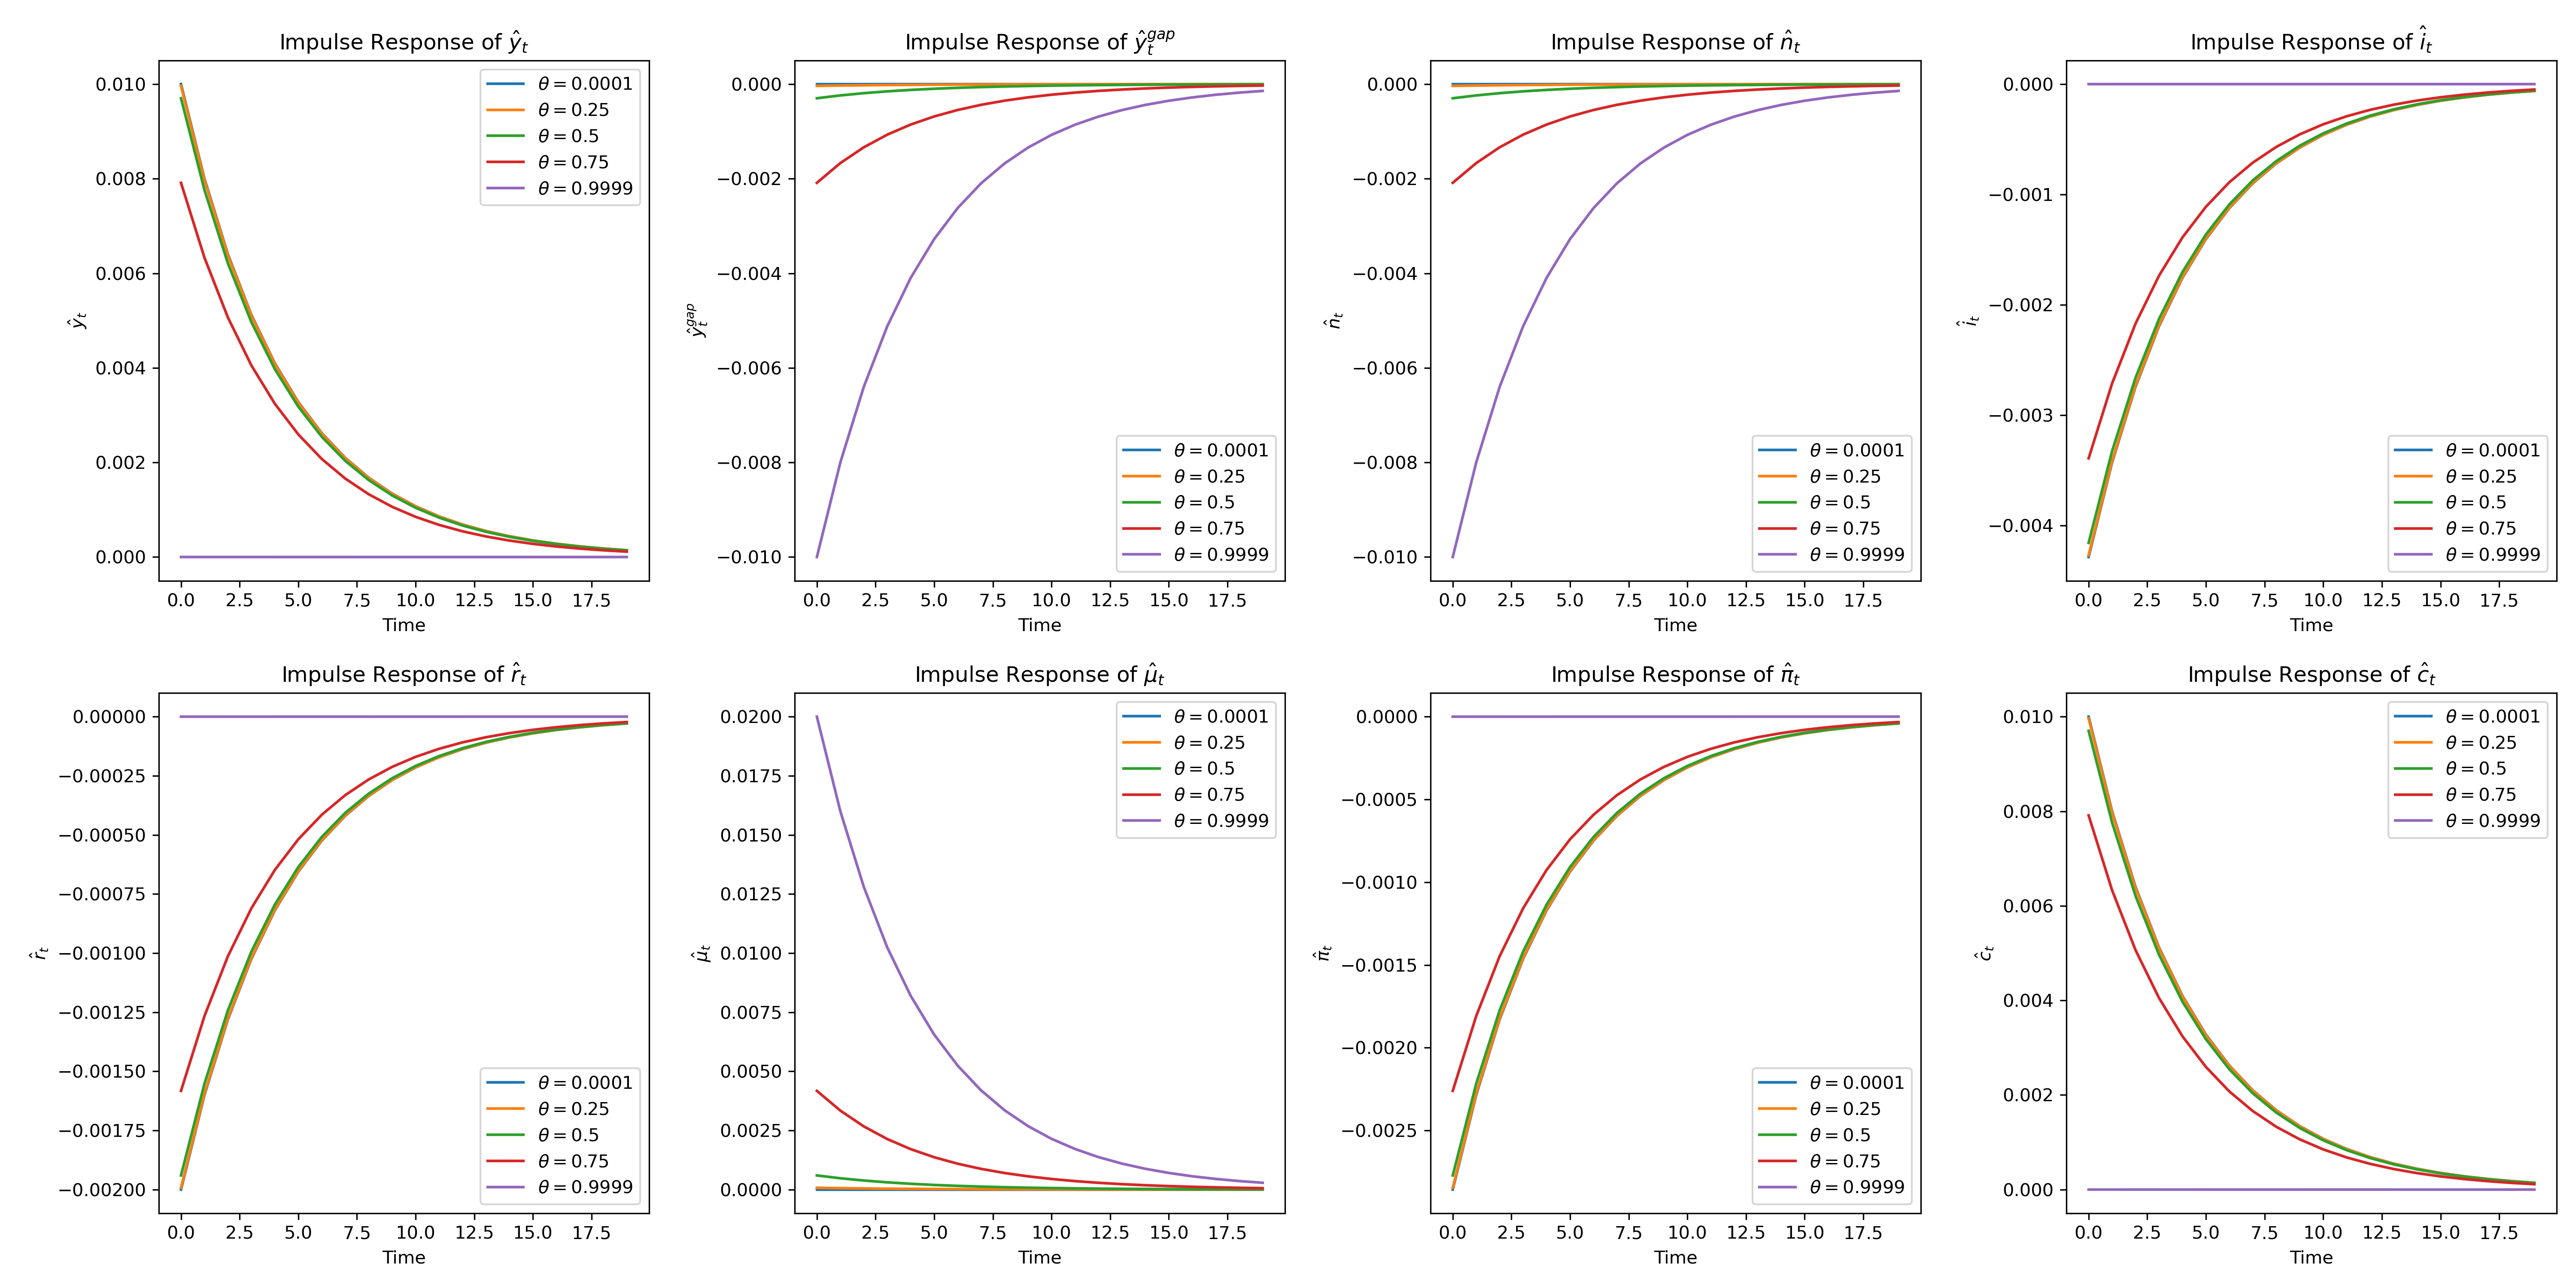
\includegraphics[width=1.0\textwidth]{figs/q2_IRFs.png}
\caption{Impulse Response Functions}
\label{fig:q2_irf}
\end{figure}

\subsection*{(h)}

Notice that $\theta$ denotes the share of intermediate firms with sticky in a given period. 
When $\theta=0.0001$. The economy is approximately frictionless, 
and when $\theta=0.9999$, the economy has very sticky prices and nearly all intermediate firms cannot adjust their prices. 

\begin{itemize}
    \item $\hat{y}_{t}$, $\hat{c}_{t}$: Higher productivity increases firms' production, which leads to increases in output and consumption.
    As $\theta$ approaches $1$, output and consumption rise less due to nominal rigidities.
    \item $\hat{y}^{gap}_{t}$: The output gap is negligible since the economy is nearly unconstrained.
    As $\theta$ approaches $1$, the output gap becomes more negative due to nominal rigidities.
    \item $\hat{n}$: There is a negligible decrease in employment because an increase in TPF leads to an increase in output with a smaller magnitude.
    As $\theta$ approaches $1$, employment tends to decline because firms can produce the same level of output with less labor input.
    \item $\hat{mc}_{t}$: There is a negligible change in the markups because the changes in labor and consumption offset.
    As $\theta$ approaches $1$, the markup goes up because firms have smaller marginal costs due to positive TFP shocks. 
    \item $\hat{\pi}_{t}$, $\hat{i}_{t}$ and $\hat{r}_{t}$: In the frictionless economy, almost all firms optimally reset their prices. So a positive TFP shock leads to a lower price level and the inflation rate decreases. The Central Bank responds by setting a lower nominal interest rate. According to the Fisher equation and by the fact that $\phi_{\pi}=1.5$, the real interest rate decreases more than the nominal interest rate.
    As $\theta$ approaches $1$, fewer firms are allowed to adjust their prices. The effects of a positive TPF shock on the three variables discussed above dissipate. 
\end{itemize}

\subsection*{(i)}

An RBC model without capital is analogous to a New Keysian model with $\theta$ approaches to $0$ where the misallocation resulting from sticky prices is eliminated. So an increase in productivity would lead to an equal amount of increase in output and consumption. Any change in nominal prices will not impact real variables. 
However, because intermediate firms have monopolist power, so in the frictionless New Keynesian model, the markup will still result in efficiency loss and the equilibrium allocation is not a first best as in RBC.  

\end{document}


